% =====================================================================
% Preliminary Results section.
%
% REQUIRES:  \usepackage{graphicx} in the preamble (standard; main.tex loads it).
% The four chart files live in proposal/figures/ (PDF, vector). If you compile
% from a different folder, adjust the figures/ path or set
%   \graphicspath{{figures/}}
% This section uses NO pgfplots and NO custom macros, so it renders as long as
% graphicx is available and the figure files are present.
% =====================================================================

\section{Preliminary Results}
\label{sec:prelim}

As a feasibility check for the proposed study (Section~\ref{sec:method}), we ran a preliminary
version of the experiment: byte-level (ByT5) and subword (mT5) students at three sizes (small, base,
large) distilled from a frozen SONAR teacher under an identical recipe on the nine study languages,
then evaluated as retrievers and scored by nDCG@10. We report five retrieval benchmarks spanning
shallow passage retrieval (Belebele), deep monolingual retrieval (MIRACL), small-pool QA (IndicQA),
and native Amharic retrieval (Amharic-PR, 2AIRTC). Two further benchmarks are deferred and reported
separately in later work: Mr.\,TyDi \citep{zhang2021mrtydi}, whose corpus-streaming cap currently
scores only a biased subset of queries, and the cross-lingual AfriCLIRMatrix, which measures a
different (query-in-English) task axis from the monolingual retrieval studied here. Across the five
benchmarks, byte embeddings win four --- losing only on the small-pool IndicQA --- and the smallest
byte model surpasses the largest subword model on every deep-retrieval benchmark
(Table~\ref{tab:prelim}). These are single-seed results at 50k steps, intended to motivate rather than
conclude the full study; absolute scores are bounded by the SONAR teacher, a bitext encoder rather
than a retriever, which the proposed retrieval-focused training is designed to lift. In every figure,
the three blue bars are byte (small/base/large) and the three amber bars are subword
(small/base/large).

\begin{table}[htbp]
\centering
\small
\begin{tabular}{l rr rr}
\toprule
& \multicolumn{2}{c}{\textbf{Students (base)}} & \multicolumn{2}{c}{\textbf{Baselines}}\\
\cmidrule(lr){2-3}\cmidrule(lr){4-5}
Benchmark (pool) & byte & subword & mE5 & LaBSE\\
\midrule
Belebele (488)        & \textbf{0.585} & 0.535 & 0.806 & 0.684\\
MIRACL ($\sim$20k)    & \textbf{0.174} & 0.064 & 0.946 & 0.522\\
IndicQA ($\sim$250)   & 0.358 & \textbf{0.503} & 0.675 & 0.490\\
Amharic-PR (20k)      & \textbf{0.470} & 0.363 & 0.333 & 0.524\\
2AIRTC (12.5k)        & \textbf{0.422} & 0.213 & 0.508 & 0.569\\
\bottomrule
\end{tabular}
\caption{Language-averaged nDCG@10 at the base size. Byte beats subword on four of five benchmarks
(bold = byte-vs-subword winner); mE5 and LaBSE are retrieval-trained reference baselines. On
Amharic-PR the distilled byte student exceeds the strong mE5 baseline.}
\label{tab:prelim}
\end{table}

\begin{figure}[htbp]
\centering
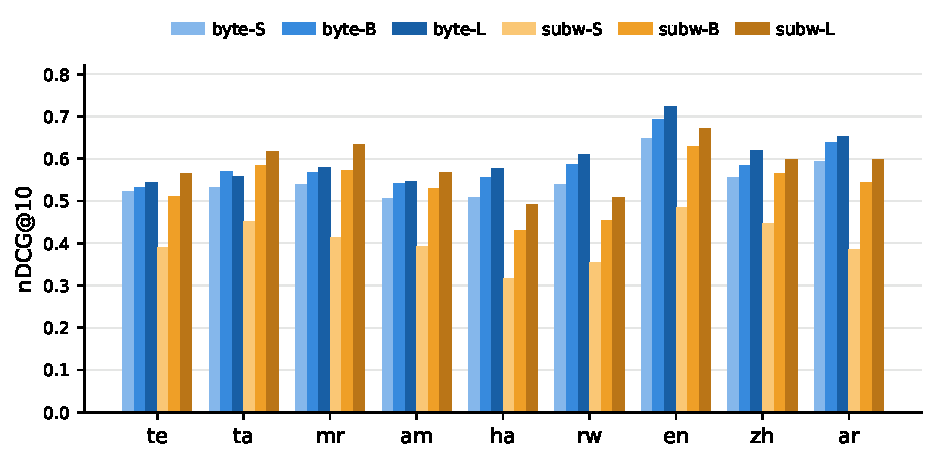
\includegraphics[width=\linewidth]{figures/fig_belebele}
\caption{\textbf{Belebele --- shallow passage retrieval (pool 488).} Byte embeddings outperform
subword at every size, with the gap largest for the smallest models and for the African languages
(Hausa, Kinyarwanda); the two families converge only at the large scale.}
\label{fig:belebele}
\end{figure}

\begin{figure}[htbp]
\centering
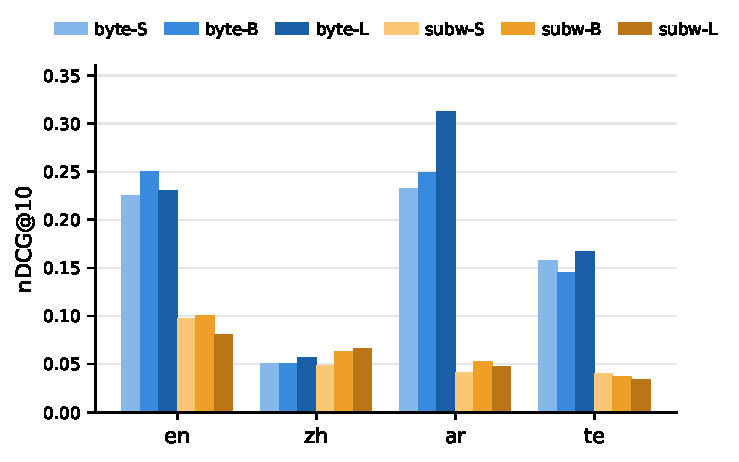
\includegraphics[width=0.72\linewidth]{figures/fig_miracl}
\caption{\textbf{MIRACL --- deep monolingual retrieval (pool $\sim$20k).} Byte beats subword by
roughly 3--5$\times$ at every size, and the smallest byte model (219M) surpasses the largest subword
model (565M); Chinese is the single hard cell for both families.}
\label{fig:miracl}
\end{figure}

\begin{figure}[htbp]
\centering
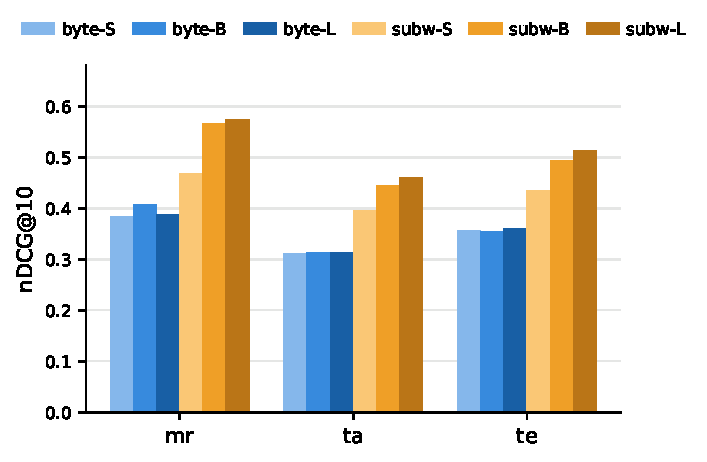
\includegraphics[width=0.64\linewidth]{figures/fig_indicqa}
\caption{\textbf{IndicQA --- small-pool QA retrieval (pool $\sim$250).} The one benchmark where
subword leads byte at every size; we attribute the reversal to the very small candidate pool, where
the larger subword vocabulary is sufficient and byte's advantage does not surface.}
\label{fig:indicqa}
\end{figure}

\begin{figure}[htbp]
\centering
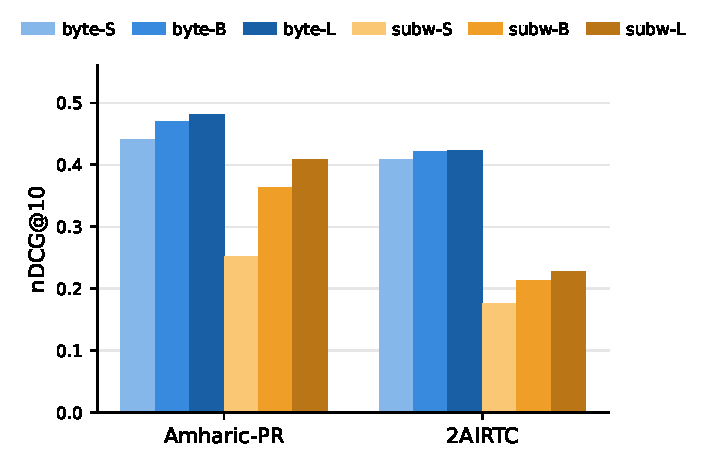
\includegraphics[width=0.56\linewidth]{figures/fig_amharic}
\caption{\textbf{Native Amharic retrieval.} On Amharic-PR (passage retrieval, pool 20k) byte leads
subword at every size and byte-base/large exceed the retrieval-trained mE5 baseline (0.47--0.48 vs
0.33). On the peer-reviewed 2AIRTC ad-hoc IR collection (pool 12.5k) byte roughly doubles subword,
corroborating the result on an independent, formally-constructed corpus.}
\label{fig:amharic}
\end{figure}

\noindent
Taken together, the preliminary run supports the central hypothesis: under a fixed distillation recipe
that varies only the tokenizer, byte embeddings are the stronger retriever for low-resource languages,
decisively so on every deep, large-pool benchmark, with the smallest byte model already outperforming
the largest subword model. The full study (Section~\ref{sec:method}) will add a retrieval-specific
training objective to raise absolute quality, multiple seeds with confidence intervals, and the
parameter-matched control to confirm the advantage is representational rather than a parameter-count
artifact.

% Flush all of this section's floats here so none drift into the bibliography that follows.
\FloatBarrier
